\documentclass[12pt,a4paper]{scrartcl}\usepackage[]{graphicx}\usepackage[]{color}
%% maxwidth is the original width if it is less than linewidth
%% otherwise use linewidth (to make sure the graphics do not exceed the margin)
\makeatletter
\def\maxwidth{ %
  \ifdim\Gin@nat@width>\linewidth
    \linewidth
  \else
    \Gin@nat@width
  \fi
}
\makeatother

\definecolor{fgcolor}{rgb}{0.345, 0.345, 0.345}
\newcommand{\hlnum}[1]{\textcolor[rgb]{0.686,0.059,0.569}{#1}}%
\newcommand{\hlstr}[1]{\textcolor[rgb]{0.192,0.494,0.8}{#1}}%
\newcommand{\hlcom}[1]{\textcolor[rgb]{0.678,0.584,0.686}{\textit{#1}}}%
\newcommand{\hlopt}[1]{\textcolor[rgb]{0,0,0}{#1}}%
\newcommand{\hlstd}[1]{\textcolor[rgb]{0.345,0.345,0.345}{#1}}%
\newcommand{\hlkwa}[1]{\textcolor[rgb]{0.161,0.373,0.58}{\textbf{#1}}}%
\newcommand{\hlkwb}[1]{\textcolor[rgb]{0.69,0.353,0.396}{#1}}%
\newcommand{\hlkwc}[1]{\textcolor[rgb]{0.333,0.667,0.333}{#1}}%
\newcommand{\hlkwd}[1]{\textcolor[rgb]{0.737,0.353,0.396}{\textbf{#1}}}%
\let\hlipl\hlkwb

\usepackage{framed}
\makeatletter
\newenvironment{kframe}{%
 \def\at@end@of@kframe{}%
 \ifinner\ifhmode%
  \def\at@end@of@kframe{\end{minipage}}%
  \begin{minipage}{\columnwidth}%
 \fi\fi%
 \def\FrameCommand##1{\hskip\@totalleftmargin \hskip-\fboxsep
 \colorbox{shadecolor}{##1}\hskip-\fboxsep
     % There is no \\@totalrightmargin, so:
     \hskip-\linewidth \hskip-\@totalleftmargin \hskip\columnwidth}%
 \MakeFramed {\advance\hsize-\width
   \@totalleftmargin\z@ \linewidth\hsize
   \@setminipage}}%
 {\par\unskip\endMakeFramed%
 \at@end@of@kframe}
\makeatother

\definecolor{shadecolor}{rgb}{.97, .97, .97}
\definecolor{messagecolor}{rgb}{0, 0, 0}
\definecolor{warningcolor}{rgb}{1, 0, 1}
\definecolor{errorcolor}{rgb}{1, 0, 0}
\newenvironment{knitrout}{}{} % an empty environment to be redefined in TeX

\usepackage{alltt}
\usepackage[utf8]{inputenc}
\usepackage{amsmath}
\usepackage{graphicx}
\usepackage{tikz}
%\usepackage{silence}
\usepackage{mdframed}
%\WarningFilter{mdframed}{You got a bad break}
\usepackage[colorinlistoftodos]{todonotes}
\usepackage{listings}
\usepackage{color}
\colorlet{exampcol}{blue!10}
\usepackage{multicol}
\usepackage{booktabs}

\usepackage{exercise}

\usepackage[autostyle, english = american]{csquotes}
\MakeOuterQuote{"}

\usepackage{hyperref}
\hypersetup{
    colorlinks,
    citecolor=black,
    filecolor=black,
    linkcolor=blue,
    urlcolor=black
}

\title{Exercises for statistical inference and stuff}
\date{\today}
\author{Timoth\'ee Bonnet}
\IfFileExists{upquote.sty}{\usepackage{upquote}}{}
\begin{document}

\begin{knitrout}
\definecolor{shadecolor}{rgb}{0.969, 0.969, 0.969}\color{fgcolor}\begin{kframe}
\begin{alltt}
\hlkwd{library}\hlstd{(lme4)}
\end{alltt}


{\ttfamily\noindent\itshape\color{messagecolor}{\#\# Loading required package: Matrix}}\begin{alltt}
\hlstd{thorns} \hlkwb{<-} \hlkwd{read.table}\hlstd{(}\hlkwc{file} \hlstd{=} \hlstr{"thorndata.txt"}\hlstd{,} \hlkwc{header}\hlstd{=}\hlnum{TRUE}\hlstd{)}
\hlstd{thornLMM} \hlkwb{<-} \hlkwd{lmer}\hlstd{(response} \hlopt{~} \hlstd{predictor} \hlopt{+} \hlstd{(}\hlnum{1}\hlopt{|}\hlstd{block),} \hlkwc{data} \hlstd{= thorns)}
\hlstd{setpar} \hlkwb{<-} \hlkwa{function}\hlstd{()}
\hlstd{\{}
\hlkwd{par}\hlstd{(}\hlkwc{las}\hlstd{=}\hlnum{1}\hlstd{,} \hlkwc{cex}\hlstd{=}\hlnum{1.2}\hlstd{)}
\hlstd{\}}
\end{alltt}
\end{kframe}
\end{knitrout}

\begin{knitrout}
\definecolor{shadecolor}{rgb}{0.969, 0.969, 0.969}\color{fgcolor}\begin{kframe}
\begin{alltt}
\hlkwd{setpar}\hlstd{()}
\hlkwd{plot}\hlstd{(thorns}\hlopt{$}\hlstd{response,} \hlkwc{x}\hlstd{=thorns}\hlopt{$}\hlstd{predictor,} \hlkwc{ylab} \hlstd{=} \hlstr{"Herbivory load"}\hlstd{,} \hlkwc{xlab}\hlstd{=} \hlstr{"Thorn density"}\hlstd{)}
\hlkwd{abline}\hlstd{(}\hlkwd{lm}\hlstd{(response}\hlopt{~} \hlstd{predictor,} \hlkwc{data}\hlstd{=thorns),} \hlkwc{lwd}\hlstd{=}\hlnum{5}\hlstd{,} \hlkwc{col}\hlstd{=}\hlstr{"gray"}\hlstd{)}\hlcom{#this is a shortcut to draw a regression line}
\end{alltt}
\end{kframe}
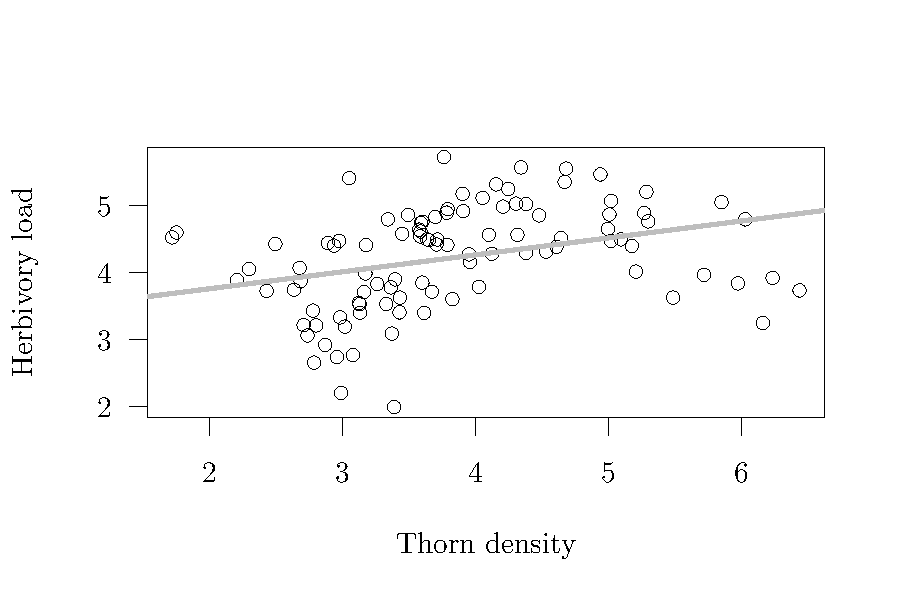
\includegraphics[width=\maxwidth]{figure/graph0-1} 

\end{knitrout}

\begin{knitrout}
\definecolor{shadecolor}{rgb}{0.969, 0.969, 0.969}\color{fgcolor}\begin{kframe}
\begin{alltt}
\hlkwd{setpar}\hlstd{()}
\hlkwd{plot}\hlstd{(thorns}\hlopt{$}\hlstd{predictor, thorns}\hlopt{$}\hlstd{response,} \hlkwc{col}\hlstd{=thorns}\hlopt{$}\hlstd{block,} \hlkwc{ylab} \hlstd{=} \hlstr{"Herbivory load"}\hlstd{,} \hlkwc{xlab}\hlstd{=} \hlstr{"Thorn density"}\hlstd{)}
\hlkwd{abline}\hlstd{(}\hlkwd{lm}\hlstd{(response}\hlopt{~} \hlstd{predictor,} \hlkwc{data}\hlstd{=thorns),} \hlkwc{lwd}\hlstd{=}\hlnum{5}\hlstd{,} \hlkwc{col}\hlstd{=}\hlstr{"gray"}\hlstd{)}
\end{alltt}
\end{kframe}
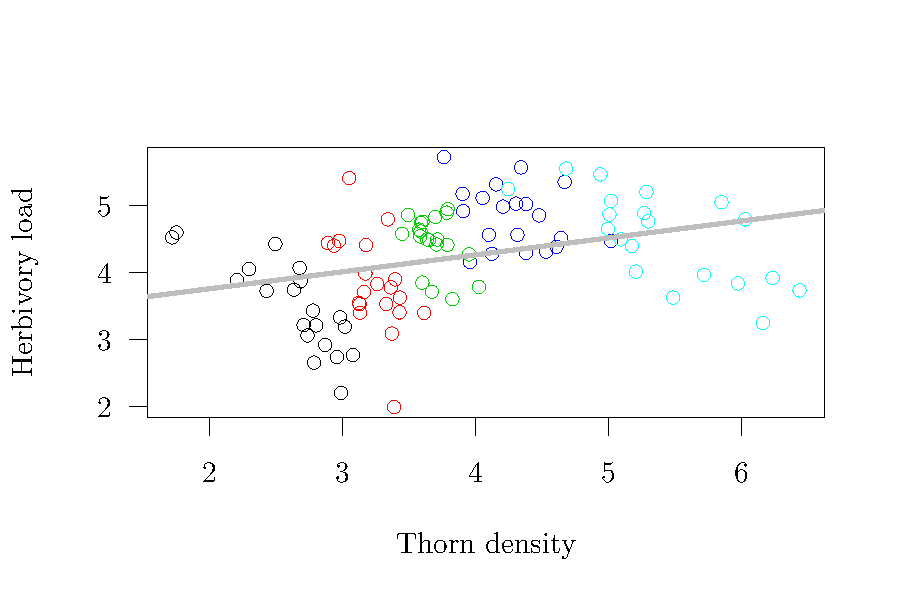
\includegraphics[width=\maxwidth]{figure/graph1-1} 

\end{knitrout}

\begin{knitrout}
\definecolor{shadecolor}{rgb}{0.969, 0.969, 0.969}\color{fgcolor}\begin{kframe}
\begin{alltt}
\hlkwd{setpar}\hlstd{()}
\hlkwd{plot}\hlstd{(thorns}\hlopt{$}\hlstd{predictor, thorns}\hlopt{$}\hlstd{response,} \hlkwc{col}\hlstd{=thorns}\hlopt{$}\hlstd{block,} \hlkwc{ylab} \hlstd{=} \hlstr{"Herbivory load"}\hlstd{,} \hlkwc{xlab}\hlstd{=} \hlstr{"Thorn density"}\hlstd{)}
\hlstd{slp} \hlkwb{<-} \hlkwd{fixef}\hlstd{(thornLMM)[}\hlnum{2}\hlstd{]}
\hlstd{inter} \hlkwb{<-} \hlkwd{fixef}\hlstd{(thornLMM)[}\hlnum{1}\hlstd{]}
\hlstd{re} \hlkwb{<-} \hlkwd{ranef}\hlstd{(thornLMM)}\hlopt{$}\hlstd{block[,}\hlnum{1}\hlstd{]}

\hlkwd{abline}\hlstd{(}\hlkwc{a} \hlstd{= inter}\hlopt{+}\hlstd{re[}\hlnum{1}\hlstd{],} \hlkwc{b}\hlstd{=slp,} \hlkwc{lwd}\hlstd{=}\hlnum{5}\hlstd{)}
\hlkwd{abline}\hlstd{(}\hlkwc{a} \hlstd{= inter}\hlopt{+}\hlstd{re[}\hlnum{2}\hlstd{],} \hlkwc{b}\hlstd{=slp,} \hlkwc{lwd}\hlstd{=}\hlnum{5}\hlstd{,} \hlkwc{col}\hlstd{=}\hlstr{"red"}\hlstd{)}
\hlkwd{abline}\hlstd{(}\hlkwc{a} \hlstd{= inter}\hlopt{+}\hlstd{re[}\hlnum{3}\hlstd{],} \hlkwc{b}\hlstd{=slp,} \hlkwc{lwd}\hlstd{=}\hlnum{5}\hlstd{,} \hlkwc{col}\hlstd{=}\hlstr{"green"}\hlstd{)}
\hlkwd{abline}\hlstd{(}\hlkwc{a} \hlstd{= inter}\hlopt{+}\hlstd{re[}\hlnum{4}\hlstd{],} \hlkwc{b}\hlstd{=slp,} \hlkwc{lwd}\hlstd{=}\hlnum{5}\hlstd{,} \hlkwc{col}\hlstd{=}\hlstr{"blue"}\hlstd{)}
\hlkwd{abline}\hlstd{(}\hlkwc{a} \hlstd{= inter}\hlopt{+}\hlstd{re[}\hlnum{5}\hlstd{],} \hlkwc{b}\hlstd{=slp,} \hlkwc{lwd}\hlstd{=}\hlnum{5}\hlstd{,} \hlkwc{col}\hlstd{=}\hlstr{"cyan"}\hlstd{)}
\end{alltt}
\end{kframe}
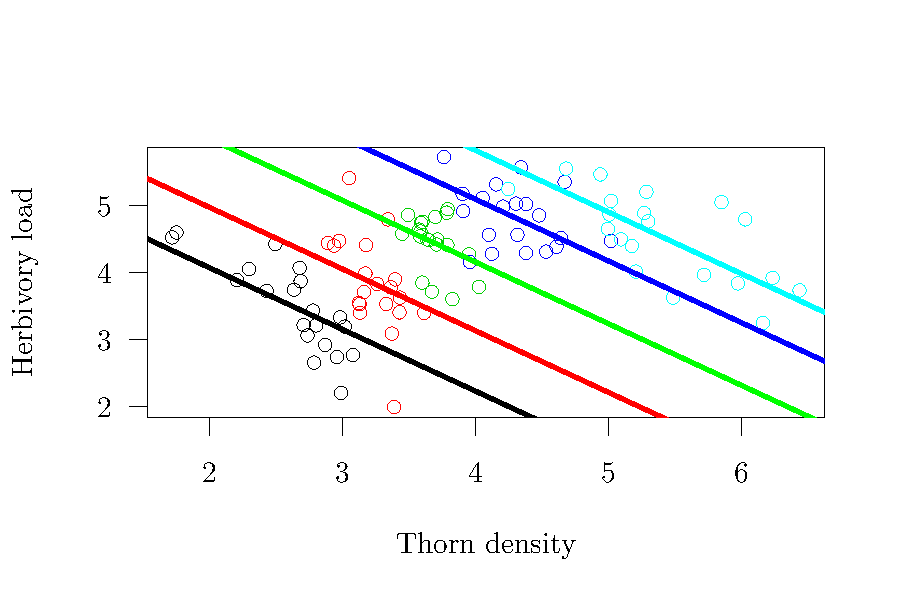
\includegraphics[width=\maxwidth]{figure/graph2-1} 

\end{knitrout}


\begin{knitrout}
\definecolor{shadecolor}{rgb}{0.969, 0.969, 0.969}\color{fgcolor}\begin{kframe}
\begin{alltt}
\hlkwd{setpar}\hlstd{()}
\hlkwd{plot}\hlstd{(thorns}\hlopt{$}\hlstd{predictor, thorns}\hlopt{$}\hlstd{response,} \hlkwc{col}\hlstd{=thorns}\hlopt{$}\hlstd{block,} \hlkwc{ylab} \hlstd{=} \hlstr{"Herbivory load"}\hlstd{,} \hlkwc{xlab}\hlstd{=} \hlstr{"Thorn density"}\hlstd{)}
\hlstd{thornLMM2} \hlkwb{<-} \hlkwd{lmer}\hlstd{(response} \hlopt{~} \hlnum{1} \hlopt{+} \hlstd{predictor} \hlopt{+} \hlstd{(}\hlnum{1}\hlopt{+}\hlstd{predictor}\hlopt{|}\hlstd{block),} \hlkwc{data}\hlstd{=thorns)}
\end{alltt}


{\ttfamily\noindent\itshape\color{messagecolor}{\#\# singular fit}}\begin{alltt}
\hlstd{slp} \hlkwb{<-} \hlkwd{fixef}\hlstd{(thornLMM2)[}\hlnum{2}\hlstd{]}
\hlstd{inter} \hlkwb{<-} \hlkwd{fixef}\hlstd{(thornLMM2)[}\hlnum{1}\hlstd{]}
\hlstd{reint} \hlkwb{<-} \hlkwd{ranef}\hlstd{(thornLMM2)}\hlopt{$}\hlstd{block[,}\hlnum{1}\hlstd{]}
\hlstd{resl} \hlkwb{<-} \hlkwd{ranef}\hlstd{(thornLMM2)}\hlopt{$}\hlstd{block[,}\hlnum{2}\hlstd{]}

\hlkwd{abline}\hlstd{(}\hlkwc{a} \hlstd{= inter}\hlopt{+}\hlstd{reint[}\hlnum{1}\hlstd{],} \hlkwc{b}\hlstd{=slp}\hlopt{+}\hlstd{resl[}\hlnum{1}\hlstd{],} \hlkwc{lwd}\hlstd{=}\hlnum{5}\hlstd{)}
\hlkwd{abline}\hlstd{(}\hlkwc{a} \hlstd{= inter}\hlopt{+}\hlstd{reint[}\hlnum{2}\hlstd{],} \hlkwc{b}\hlstd{=slp}\hlopt{+}\hlstd{resl[}\hlnum{2}\hlstd{],} \hlkwc{lwd}\hlstd{=}\hlnum{5}\hlstd{,} \hlkwc{col}\hlstd{=}\hlstr{"red"}\hlstd{)}
\hlkwd{abline}\hlstd{(}\hlkwc{a} \hlstd{= inter}\hlopt{+}\hlstd{reint[}\hlnum{3}\hlstd{],} \hlkwc{b}\hlstd{=slp}\hlopt{+}\hlstd{resl[}\hlnum{3}\hlstd{],} \hlkwc{lwd}\hlstd{=}\hlnum{5}\hlstd{,} \hlkwc{col}\hlstd{=}\hlstr{"green"}\hlstd{)}
\hlkwd{abline}\hlstd{(}\hlkwc{a} \hlstd{= inter}\hlopt{+}\hlstd{reint[}\hlnum{4}\hlstd{],} \hlkwc{b}\hlstd{=slp}\hlopt{+}\hlstd{resl[}\hlnum{4}\hlstd{],} \hlkwc{lwd}\hlstd{=}\hlnum{5}\hlstd{,} \hlkwc{col}\hlstd{=}\hlstr{"blue"}\hlstd{)}
\hlkwd{abline}\hlstd{(}\hlkwc{a} \hlstd{= inter}\hlopt{+}\hlstd{reint[}\hlnum{5}\hlstd{],} \hlkwc{b}\hlstd{=slp}\hlopt{+}\hlstd{resl[}\hlnum{5}\hlstd{],} \hlkwc{lwd}\hlstd{=}\hlnum{5}\hlstd{,} \hlkwc{col}\hlstd{=}\hlstr{"cyan"}\hlstd{)}
\end{alltt}
\end{kframe}
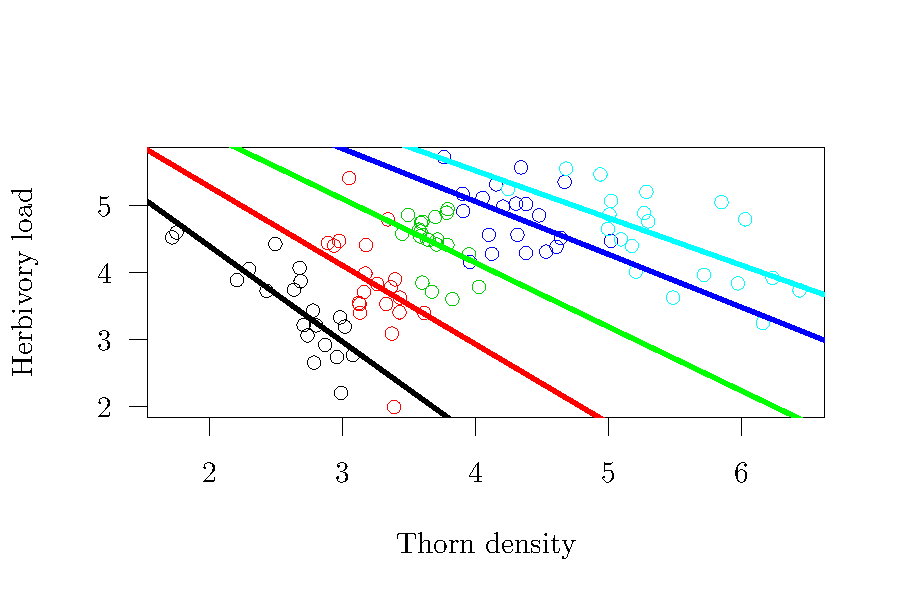
\includegraphics[width=\maxwidth]{figure/graphrslopes-1} 

\end{knitrout}
\end{document}
